\documentclass[]{scrbook}
\KOMAoptions
{
	fontsize=14pt,
	paper=14.8cm:14.8cm,
	pagesize=pdftex,
	BCOR=0.0mm,
	DIV=15,
	twoside=false
}
\usepackage[ngerman]{babel}
\usepackage{tikz}

\usetikzlibrary{arrows,shapes,positioning,arrows.meta}
\definecolor{shamrock}{RGB}{46, 204, 113}
\definecolor{monza}{RGB}{207, 0, 15}
\definecolor{dolly}{RGB}{247, 202, 24}
\definecolor{silver}{RGB}{108, 122, 137}
\definecolor{rand}{RGB}{0,0,115}
\definecolor{hellblau}{RGB}{99,237,255}
\tikzset{greenvector/.style={-{Triangle[fill=shamrock]},thick,white,double=shamrock,double distance = 4pt}}
\tikzset{redvector/.style={-{Triangle[fill=monza]},thick,white,double=monza,double distance = 4pt}}
\tikzset{yellowvector/.style={-{Triangle[fill=dolly]},thick,white,double=dolly,double distance = 4pt}}


\usepackage[OT1]{fontenc}
\renewcommand*\familydefault{\sfdefault}

\pagestyle{empty}



\begin{document}
\begin{tikzpicture}[remember picture,overlay]
 \node[opacity=1.0,inner sep=0pt] at (current page.center){\includegraphics[width=\paperwidth,height=\paperheight]{4-01.eps}
};
\end{tikzpicture}
\begin{tikzpicture}[remember picture,overlay]
\node[white] at (6,0.5) {\small Gerrit Herrmann};
\node[rand] at (2.5,-1.5) {\Huge\bfseries Lineare Algebra};
\node[rand] at (5.5,-11.5) {\Huge\bfseries für Babys};
\node[cloud,line width=4, draw=rand, fill=white, minimum width=100,minimum height=80,cloud puffs=11] at (7.75,-2) {};
\node[inner sep=0pt] at (7.75,-1.9) {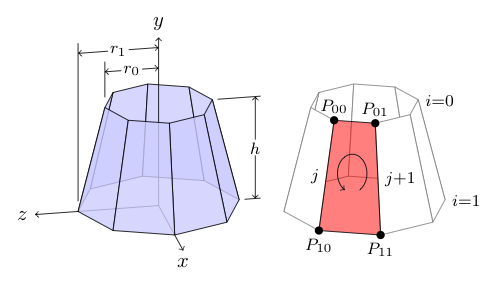
\includegraphics[scale=0.35]{3d-cone.pdf}};
\draw[line width=4,rand] (5.5,-2.5) circle (7.5pt);
\draw[line width=4,rand] (5,-3) circle (5pt);
\filldraw[white] (5.5,-2.5) circle (7.5pt);
\filldraw[white] (5,-3) circle (5pt);
\end{tikzpicture}
\bfseries
\begin{center}
	\clearpage
	\begin{tikzpicture}
		\draw[black] (-4,-2) rectangle (8,8);
		\draw[greenvector] (0,0) -- (5,3);
	\end{tikzpicture}\\
Das ist ein \textcolor{shamrock}{Vektor}. \clearpage
	\begin{tikzpicture}
	\draw[black] (-4,-2) rectangle (8,8);
	\draw[greenvector] (0,0) -- (5,3);
	\draw[silver,thick] (0,0) circle (1);
	\fill[silver] (0,0) circle (0.1);
\end{tikzpicture}\\
Ein Vektor hat einen Anfang ...  \clearpage
	\begin{tikzpicture}
	\draw[black] (-4,-2) rectangle (8,8);
	\draw[greenvector] (0,0) -- (5,3);
		\draw[silver,thick] (5,3) circle (1);
	\fill[silver] (5,3) circle (0.1);
\end{tikzpicture}\\
...\ und ein Vektor hat ein Ende. \clearpage
	\begin{tikzpicture}
		\draw[black] (-4,-2) rectangle (8,8);
	\draw[greenvector] (0,0) -- (7.5,4.5);
\end{tikzpicture}\\
Einen Vektor kann man verlängern. \clearpage
	\begin{tikzpicture}
		\draw[black] (-4,-2) rectangle (8,8);
	\draw[greenvector] (0,0) -- (2.5,1.5);
\end{tikzpicture}\\
Einen Vektor kann man kürzen. \clearpage
	\begin{tikzpicture}
			\draw[black] (-4,-2) rectangle (8,8);
	\draw[greenvector] (5,3) -- (0,0);
\end{tikzpicture}\\
Man kann einen Vektor auch umdrehen. \clearpage
	\begin{tikzpicture}
		\draw[black] (-4,-2) rectangle (8,8);
	\draw[-{Triangle[fill=monza]}, thick,white,double=monza,double distance = 4pt] (0,0) -- (1,4);
\end{tikzpicture}\\
Dies ist ein anderer \textcolor{monza}{Vektor}.\clearpage
	\begin{tikzpicture}
	\draw[black] (-4,-2) rectangle (8,8);
	\draw[-{Triangle[fill=monza]}, thick,white,double=monza,double distance = 4pt] (0,0) -- (2,7.5);
\end{tikzpicture}\\
Auch den kann man verlängern ...\clearpage
	\begin{tikzpicture}
	\draw[black] (-4,-2) rectangle (8,8);
	\draw[-{Triangle[fill=monza]}, thick,white,double=monza,double distance = 4pt] (0,0) -- (0.5,2);
\end{tikzpicture}\\
... und kürzen.\clearpage
	\begin{tikzpicture}
			\draw[black] (-4,-2) rectangle (8,8);
	\draw[redvector] (0,0) -- (1,4);
\end{tikzpicture}\\
Man kann an den \textcolor{monza}{roten} Vektor ... \clearpage
\begin{tikzpicture}
	\draw[black] (-4,-2) rectangle (8,8);
	\draw[redvector] (0,0) -- (1,4);
	\draw[greenvector] (1,4) -- (6,7);
\end{tikzpicture}\\
... den \textcolor{shamrock}{grünen} Vektor legen. \clearpage
	\begin{tikzpicture}
		\draw[black] (-4,-2) rectangle (8,8);
	\draw[redvector] (0,0) -- (1,4);
	\draw[greenvector] (1,4) -- (6,7);
		\draw[yellowvector] (0,0) -- (6,7);
\end{tikzpicture}\\
Dadurch erhält man einen neuen \textcolor{dolly}{Vektor}. \clearpage
	\begin{tikzpicture}
			\draw[black] (-4,-2) rectangle (8,8);
	\draw[greenvector] (0,0) -- (5,3);
\end{tikzpicture}\\
Man kann auch an den \textcolor{shamrock}{grünen} Vektor ...\clearpage
	\begin{tikzpicture}
			\draw[black] (-4,-2) rectangle (8,8);
	\draw[greenvector] (0,0) -- (5,3);
	\draw[redvector] (5,3) -- (6,7);
\end{tikzpicture}\\
... den \textcolor{monza}{roten} Vektor legen. \clearpage
	\begin{tikzpicture}
	\draw[black] (-4,-2) rectangle (8,8);
	\draw[greenvector] (0,0) -- (5,3);
	\draw[redvector] (5,3) -- (6,7);
		\draw[yellowvector] (0,0) -- (6,7);
\end{tikzpicture}\\
Damit erhält man wieder einen \textcolor{dolly}{Vektor}.\clearpage
	\begin{tikzpicture}

	\draw[black] (-4,-2) rectangle (8,8);
	\draw[redvector] (0,0) -- (1,4);
	\draw[greenvector] (1,4) -- (6,7);
	\draw[greenvector] (0,0) -- (5,3);
	\draw[redvector] (5,3) -- (6,7);
		\draw[yellowvector] (0,0) -- (6,7);
	\draw[silver,thick] (0,0) circle (1);
	\fill[silver] (0,0) circle (0.1);
	\draw[silver,thick] (6,7) circle (1);
	\fill[silver] (6,7) circle (0.1);
\end{tikzpicture}\\
Beide Fälle haben den gleichen Anfangs- und Endpunkt und somit sind die \textcolor{dolly}{Vektoren} gleich.\clearpage
	\begin{tikzpicture}
	\draw[black] (-4,-2) rectangle (8,8);
	\draw[greenvector] (0,0) -- (2.5,1.5);
	\draw[redvector] (2.5,1.5) -- (3,3.5);
	\draw[yellowvector] (0,0) -- (3,3.5);
\end{tikzpicture}\\
Wenn man den \textcolor{shamrock}{grünen}, \textcolor{monza}{roten} und \textcolor{dolly}{gelben} Vektor gleich viel kürzt, ...\clearpage
	\begin{tikzpicture}
	\draw[black] (-4,-2) rectangle (8,8);
	\draw[greenvector] (0,0) -- (2.5,1.5);
	\draw[redvector] (2.5,1.5) -- (3,3.5);
	\draw[yellowvector] (0,0) -- (3,3.5);
	\draw[silver,thick] (0,0) circle (1);
	\fill[silver] (0,0) circle (0.1);
	\draw[silver,thick] (3,3.5) circle (1);
	\fill[silver] (3,3.5) circle (0.1);
\end{tikzpicture}\\
... dann hat die Verbindung aus \textcolor{shamrock}{grün} und \textcolor{monza}{rot} immer noch den gleichen Anfangs- und Endpunkt wie \textcolor{dolly}{gelb}.   \clearpage
	\begin{tikzpicture}
	\draw[black] (-4,-2) rectangle (8,8);
	\draw[greenvector] (0,0) -- (5,3);
	\draw[redvector] (0,0) -- (1,4);
	\draw[yellowvector] (0,0) -- (6,7);
\end{tikzpicture}\\
Alle Vektoren zusammen mit diesen Eigenschaften nennt man einen Vektorraum.\clearpage
\Huge Herzlichen Glückwunsch! \\
\vspace{0.7cm}
\begin{tikzpicture}
	\node at (0,0) {};
	\begin{scope}[yshift=-1]
		\node[opacity=1,inner sep=0pt] at (0,0){\includegraphics[scale=0.25]{334.eps}
		};
	\end{scope}
\end{tikzpicture}\\
Du bist jetzt Algebraiker.\clearpage
\pagecolor{hellblau}
\topskip0pt
\vspace*{\fill}
\normalsize\color{rand} Für Frederik und Marit. \\
Für die zwei besten Geschenke der Welt. \\
Damit Ihr immer Spa\ss\ am Lernen habt und mit Neugier die Welt entdeckt.\\
\end{center}
\vspace*{\fill}
\tiny Bilder: Freepik.com. Das Cover und die vorletzte Seite wurden mit Ressourcen von Freepik.com erstellt. \\
Bild in der Traumwolke im Cover: https://texample.net/tikz/examples/3d-cone/ 

\end{document}
